\documentclass[conference]{IEEEtran}
\usepackage{cite}
\usepackage{amsmath,amssymb,amsfonts}
\usepackage{algorithmic}
\usepackage{graphicx}
\usepackage{textcomp}
\usepackage{xcolor}
\def\BibTeX{{\rm B\kern-.05em{\sc i\kern-.025em b}\kern-.08em
    T\kern-.1667em\lower.7ex\hbox{E}\kern-.125emX}}
\begin{document}

\title{Servicios Cognitivos y su Impacto en la Gestión del Conocimiento}

\author{\IEEEauthorblockN{Danny Goicochea Mendo}
\IEEEauthorblockA{\textit{Escuela de Postgrado} \\
\textit{UPAO}\\
Trujillo, Perú \\
dgoicocheam1@upao.edu.pe}
\and
\IEEEauthorblockN{Borys Rojas Jaramillo}
\IEEEauthorblockA{\textit{Escuela de Postgrado} \\
\textit{UPAO}\\
Trujillo, Perú \\
brojasj1@upao.pe}
\and
\IEEEauthorblockN{Enrique Aquino Rojas}
\IEEEauthorblockA{\textit{Escuela de Postgrado} \\
\textit{UPAO}\\
Trujillo, Perú \\
daquinor@upao.pe}
\and
\IEEEauthorblockN{Luis Canaval Sánchez}
\IEEEauthorblockA{\textit{Escuela de Postgrado} \\
\textit{UPAO}\\
Trujillo, Perú \\
lcanavals@upao.edu.pe}
}

\maketitle

\begin{abstract}
Este artículo tiene como objetivo comprender los servicios cognitivos en el ámbito tecnológico y empresarial y su impacto en la gestión del conocimiento para fines académicos y sociales. Los resultados nos permiten concluir que estos servicios cognitivos, no solo están siendo explotados a nivel tecnológico por las grandes corporaciones a nivel comercial, sino también existen servicios open source al alcance de todos y cuyo impacto en la gestión del conocimiento se traduce en creación de agentes de cambio no solo por el uso del conocimiento como información en una organización, sino que puede ser explotada para llegar a un nivel de generación de nuevo conocimiento que genere un valor competitivo ya sea a nivel de procesos, tiempos de respuesta en acceso  a la información y su valor intrínseco en la toma de decisiones.
\end{abstract}

\begin{IEEEkeywords}
cognitive services, knowledge management
\end{IEEEkeywords}

\section{Introducción}

La gestión del conocimiento es una disciplina en proceso de adopción por un gran numero de
empresas, organizaciones e instituciones, cuyo proceso es arduo y demanda una gran inversión de
recursos. Por otro lado, los sistemas cognitivos, como un producto orientado a simplificar la
aplicación de poderosos conceptos de inteligencia artificial para el procesamiento de datos, se
presentan como el siguiente paso en la evolución natural de la industria en general. Servicios
como Azure Cognitive Search o IBM Watson Discovery \cite{Tadejko2020}, ganan cada vez
más clientes con el pasar de los recientes años. El presente estudio busca resaltar el impacto
que ha tenido la adopción de servicios cognitivos de diversa índole, en las distintas etapas de
la gestión del conocimiento como un proceso continuo. Investigamos casos de aplicación de
servicios cognitivos en empresas y resaltamos el impacto positivo obtenido.

En la sección II describimos conceptos importantes para el mejor entendimiento del presente
estudio, en la sección III presentamos algunos casos de aplicación donde destacamos el impacto
logrado, en la sección IV presentamos datos del uso de servicios cognitivos para la gestión del
conocimiento, en la sección V discutimos posibles nichos de aplicación de servicios cognitivos
como parte integral de la gestión del conocimiento, finalmente en la sección VI presentamos
nuestras conclusiones \cite{Ogiela2018}.
\section{Marco Teórico}

\subsection{Servicios Cognitivos}

Los servicios cognitivos (Cognitive Services) ponen la inteligencia artificial al alcance de todos los profesionales sin que para utilizarla sea necesario contar con experiencia aprendizaje máquina (Machine Learning) a nivel técnico. Basta con una llamada a una API para incorporar la capacidad de ver, escuchar, hablar, buscar, comprender y potenciar la toma de decisiones en las aplicaciones \cite{Shwartz2019}.

Los servicios cognitivos permiten dotar a los sistemas informáticos de diversa índole, de las capacidades que tenemos los humanos de percibir y procesar aquello que ha sido percibido, apoyándose en las capacidades que proporciona el aprendizaje máquina. La tecnología cuenta con la ventaja de que la tecnología no sufre de errores por cansancio o aburrimiento ante tareas repetitivas, y por lo tanto son capaces de realizar muchos trabajos en mejores condiciones que su equivalente humano. Gracias a los servicios cognitivos es posible dotar cualquier producto de inteligencia artificial sin contar con un equipo de expertos en aspectos técnicos de alta complejidad.

\subsection{Azure Cognitive Service}

Los servicios cognitivos son una serie de servicios en forma de API REST creadas por Microsoft que nos facilitan el uso de la Inteligencia artificial de una manera fácil y directa a todas nuestras aplicaciones \cite{Brusakova2020}.

Estos servicios se dividen en cinco grandes categorías que son:

\subsubsection{Visión} Las APIs de esta categoría nos ayudan a identificar cosas tales como objetos o caras (reconocimiento facial) dentro de imágenes. También nos permiten identificar emociones (contento, enfadado, disgustados, etc.) tanto en imágenes como en videos con caras.

\subsubsection{Voz} Estas APIs de voz nos permiten hacer cosas tales como convertir el texto en voz y viceversa. Por ejemplo, también podemos usar en concreto la API Speaker Recognition API para identificar y verificar voces y usarlo dentro de nuestros en sistemas de autenticación (reconocer la voz de una persona para darle acceso a una aplicación, por ejemplo).

\subsubsection{Conocimiento}: Estas APIs nos permiten por ejemplo recomendar productos a clientes dependiendo de la actividad pasada del usuario, en el caso por ejemplo de que tuviéramos una tienda online. También nos pueden ayudar a extraer información relevante dentro de textos.

\subsubsection{Búsqueda} Estas APIs nos proporcionan capacidades de búsqueda dentro de nuestras aplicaciones usando como motor Bing.com. Estas APIs nos pueden ayudar en cosas como la búsqueda de imágenes, noticias, videos y páginas web.

\subsubsection{Lenguaje} Estas APIs nos pueden ayudar a realizar cosas como corrección gramatical y ortográfica de textos. También podemos usarlas para extraer análisis del sentimiento de textos o incluso cosas tales como detectar texto dentro de escritos a mano \cite{Ogiela2018}.

Una de las API más importantes es LUIS (Language Understanding Intelligent Service), que nos permite incluir en nuestras aplicaciones en las que el usuario se comunica con nosotros a través de una conversación, poder entender qué acciones quiere realizar el usuario en nuestras aplicaciones. Decir que esta API es el compañero perfecto en el desarrollo de chatbots, en el que el medio de comunicarse el usuario con nuestra aplicación es a través de conversaciones.


\section{Casos de éxito}
Tal crecimiento sin precedentes de la IoT, los dispositivos de interacción y la adopción de la computación móvil requiere marcos de toma de decisiones y computación basados en datos inteligentes para abstraer estos datos de sensores sin procesar, heterogéneos pero complementarios, en información procesable y conocimiento significativo. Los últimos años han visto un tremendo crecimiento en la investigación de IA que, en parte, ha sembrado e impulsado el surgimiento de varios servicios cognitivos como dominio mediador entre la IA y los datos de IoT para aprovechar y desplegar la riqueza de la información para lograr la naturalidad y la sincronicidad de los medios.
Por ello se tiene que los servicios cognitivos se pueden agrupar en términos generales en cinco categorías: lenguaje, habla, visión, conocimiento y búsqueda. Los ejemplos de cada categoría incluyen: 1) los servicios lingüísticos se denominan reconocimiento y vinculación de entidades, análisis de opiniones y clasificación de intenciones; 2) servicios de voz tales como conversión de voz a texto y viceversa; 3) servicios de visión, por ejemplo, reconocimiento facial y subtítulos automáticos de imágenes; 4) conocimientos tales como análisis de datos y descubrimiento de noticias; y 5) búsqueda como sugerencia automática, imagen, noticias, video y búsqueda web.  Figura 2 muestra
 cómo un chatbot básico se puede ampliar con varios servicios cognitivos en línea para lograr una inteligencia similar a la humana. Si bien los servicios Cognitivos de Watson de IBM se muestran en estos ejemplos, ahora hay disponibles conjuntos crecientes de servicios alternativos \cite{Molnar2019}.

\begin{figure}[htbp]
\centerline{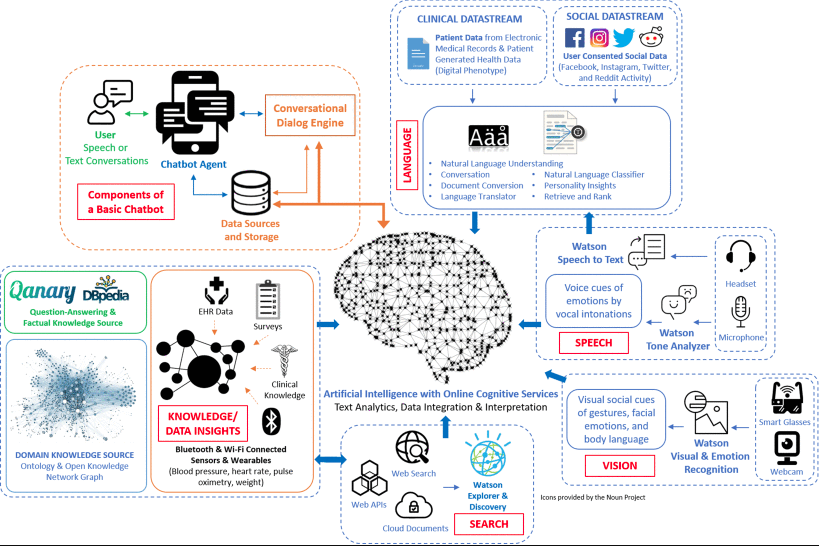
\includegraphics[width = 0.5 \textwidth]{fig02.png}}
\caption{Ilustración de cómo se puede ampliar un chatbot básico utilizando un conjunto de servicios cognitivos de ejemplo.}
\label{fig2}
\end{figure}
{\color{red}}

Las principales empresas tecnológicas (Amazon, Facebook e IBM) se han embarcado en el uso de la tecnología de voz. Si bien el éxito hasta ahora es modesto, las conversaciones de voz atractivas (en lugar de texto) en el chatbot son una promesa importante para la futura interacción hombre-máquina. Si bien los chatbots contemporáneos de propósito general han tenido un éxito limitado principalmente debido a la fragilidad en el contexto del modelado y la capacidad de utilizar un conocimiento más amplio, los chatbots en un dominio como el de la atención médica son muy prometedores y están recibiendo un gran interés correspondiente. Esto se debe en parte a la capacidad de utilizar datos multimodales y el acceso al conocimiento estructurado de la medicina, como lo demuestran las aplicaciones digitales de salud personalizadas para el asma y las enfermedades cardiovasculares. [9] , [10]Con el uso de IoT ampliado con un conjunto de servicios cognitivos, como se ilustra en la Figura 2 , para proporcionar el contexto circundante, las conversaciones de chatbot se pueden hacer más sólidas y significativas. La siguiente sección ilustra cómo los servicios cognitivos en línea pueden aprovechar los datos multimodales para brindar acceso e integración con los dominios de atención médica \cite{Majarres}.

\subsection{Integracin con dominios de salud}

Si bien la alimentación de datos sin procesar generados a partir de IoT en varias canalizaciones de servicios cognitivos en línea para traducirlos en información significativa es un paso más cerca de los chatbots inteligentes, creemos que también es importante que el sistema combine, desmitifique y dé sentido a estos datos a través de la contextualización, personalización y abstracción. Contextualización se refiere a la interpretación de datos en términos de conocimiento (contexto). Por lo general, se refiere al mapeo de datos detallados que cubren varias facetas mediante la determinación del tipo y el valor de los datos, y luego los ubica en relación con otros conceptos de dominio, lo que deriva en una interpretación significativa de los resultados. Como ejemplo, un chatbot contextualizado con conocimiento del dominio puede comprender los términos de la jerga que se usan comúnmente en las redes sociales, como "bupe", que se refiere a su jerga médica "buprenorfina" \cite{Rojas}. Personalización se refiere al curso de acción futuro teniendo en cuenta varios factores con respecto a un paciente en particular, como el historial de salud, las características físicas, el entorno, la actividad y el estilo de vida. Por ejemplo, un chatbot contextualizado y personalizado puede indicar el clima con respecto a la vulnerabilidad de un paciente asmático a un alto nivel de polen de ambrosía y sugerir acciones apropiadas. Abstracciónes una técnica computacional que mapea y asocia datos sin procesar con información relacionada con la acción para proporcionar una vista integrada de las medidas de remediación adecuadas. Por ejemplo, una alta actividad diaria en el contexto de la salud puede abstraerse y traducirse en un bajo riesgo de problemas cardíacos según la información demográfica y genética, así como la dieta. Para pintar una perspectiva más granular, a continuación se ilustran algunos casos de uso sobre cómo estos chatbots inteligentes que aprovechan los servicios cognitivos en línea se pueden usar como un "entrenador de salud personal" en los dominios de atención médica.

Como instancias de chatbots inteligentes creados con servicios cognitivos, describimos tres chatbots inteligentes en desarrollo en proyectos financiados por NIH sobre depresión/salud mental ( http://bit.ly/depression-social ), asma pediátrica ( http://bit.ly /kSalud-Asma), y cuidado de ancianos. En el caso de la enfermedad mental, la detección convencional a menudo administra Cuestionarios de Salud del Paciente (PHQ-9) para evaluar la gravedad de la depresión del paciente. Sin embargo, tal cribado tiene dos defectos inherentes. Se basa en gran medida en la capacidad del paciente para recordar eventos que ocurrieron durante las últimas dos semanas, y todos los criterios del PHQ-9 tienen el mismo peso. Por ejemplo, el criterio “sentirse cansado o tener poca energía” se pondera de manera similar a los “pensamientos de que estaría mejor muerto o lastimarse a sí mismo de alguna manera”. Un chatbot inteligente tiene la capacidad de aprovechar varios dispositivos IoT y servicios cognitivos en línea, como una cámara para evaluar el estado de ánimo actual de un paciente a través del reconocimiento visual; el micrófono que aprovecha el servicio de analizador de tono para analizar la tonalidad y el sentimiento del habla; servicio de insights de personalidad para determinar la personalidad del paciente; acceso a los perfiles consentidos del paciente para descubrir manifestaciones de comportamiento y calumnias en varias plataformas de redes sociales; comprensión de idiomas y servicios de traducción para el análisis lingüístico, como el uso de términos de argot; y QnA maker para formular preguntas inteligentes. Una combinación de estos servicios cognitivos en línea puede superar la naturaleza transitoria del recuerdo de la memoria y capturar cambios de comportamiento sutiles que de otro modo se pasarían por alto o no se traducirían de manera evidente durante la evaluación de PHQ-9. Estos permiten además una entrada viable para la entrega de psicoterapia de acuerdo con la terapia cognitivo-conductual. comprensión de idiomas y servicios de traducción para el análisis lingüístico, como el uso de términos de argot; y QnA maker para formular preguntas inteligentes. Una combinación de estos servicios cognitivos en línea puede superar la naturaleza transitoria del recuerdo de la memoria y capturar cambios de comportamiento sutiles que de otro modo se pasarían por alto o no se traducirían de manera evidente durante la evaluación de PHQ-9. Estos permiten además una entrada viable para la entrega de psicoterapia de acuerdo con la terapia cognitivo-conductual. comprensión de idiomas y servicios de traducción para el análisis lingüístico, como el uso de términos de argot; y QnA maker para formular preguntas inteligentes. Una combinación de estos servicios cognitivos en línea puede superar la naturaleza transitoria del recuerdo de la memoria y capturar cambios de comportamiento sutiles que de otro modo se pasarían por alto o no se traducirían de manera evidente durante la evaluación de PHQ-9. Estos permiten además una entrada viable para la entrega de psicoterapia de acuerdo con la terapia cognitivo-conductual.[11] e iniciar la necesidad de una intervención de tratamiento conforme a los protocolos médicos.

En el caso de la enfermedad del asma, el diagnóstico tradicional, como la prueba de control del asma, generalmente se centra y se limita a la información disponible del paciente al médico en el momento de las visitas al hospital. Hay tantos conocimientos que se pueden obtener de datos tan limitados. Un chatbot inteligente, por el contrario, es capaz de llenar y cerrar este vacío de información. Por ejemplo, puede aprovechar los servicios en línea para datos meteorológicos y registros médicos electrónicos (analizados mediante servicios cognitivos como conversión de documentos, clasificación y comprensión del lenguaje natural) para comprender la susceptibilidad del paciente al polen de ambrosía, combinar estos tipos individuales de información y sugerir cursos apropiados. de acciones Imagine dos respuestas diferentes para la misma consulta que busca información meteorológica, “Puede esperar un clima bastante soleado hoy” y “Puede esperar un clima bastante soleado hoy, sin embargo, el nivel de polen de ambrosía es un poco alto, lo que no parece bueno para su condición de asma. Minimice cualquier actividad al aire libre”. La primera es una tarea de recuperación de información sin capacidad cognitiva, mientras que la segunda representa capacidades de razonamiento contextualizado, inferencia y recomendación que pueden enriquecer la calidad de vida del paciente.

En el caso del cuidado de ancianos, además de residir con un mayor riesgo de desarrollar enfermedades crónicas, los residentes mayores a menudo caen en los grupos de analfabetos y escépticos tecnológicos en comparación con sus compatriotas más jóvenes ( http://bit.ly/Elder-Technology). Un chatbot proporciona una barrera de entrada más baja para los ancianos que adoptan el uso de la tecnología. Como ejemplo ortogonal, un chatbot equipado con reconocimiento de voz, traducción multilingüe y servicios cognitivos de comprensión del lenguaje natural permite a las personas mayores con problemas de alfabetización enviar mensajes de texto o hablar, lo que sea con lo que se sientan más cómodos. Alternativamente, un chatbot con acceso a API geográficas, locales y web también es capaz de brindar apoyo social, como organizar sesiones de telesalud, programar citas médicas y coordinar y organizar servicios de transporte para personas mayores con discapacidades físicas y barreras de transporte, especialmente en ciudades congestionadas. Sin embargo, tales capacidades y funcionalidades ilustradas solo han arañado la superficie de los posibles casos de uso más amplios de servicios cognitivos en línea para chatbots inteligentes. Su impacto emergente y su perfecta integración en la prestación de atención médica para una salud personalizada aumentada[12] tales como el autocontrol, la autoevaluación, el autocontrol, la intervención y la proyección del riesgo y la progresión de la enfermedad de deben promover y aprovechar, de acuerdo con los mejores intereses tanto del paciente como del médico.

Hemos seleccionado cuatro artículos que cumplieron con los estándares de alta calidad para este número especial. Estos documentos describieron las diversas dimensiones de un chatbot inteligente, que van desde la gestión del diálogo hasta las aplicaciones del mundo real y cómo puede causar daño si se abusa de manera inapropiada.

En "Enfoques para la gestión del diálogo en agentes conversacionales", Jan-Gerrit Harms et al.examinó el campo de la gestión del diálogo y estableció una visión general de las formas en que se ha abordado el diálogo. Luego, los autores taxonomizaron, compararon y contrastaron varias herramientas de administración de diálogos, incluidos enfoques artesanales (basados en reglas), probabilísticos (estadísticos) e híbridos en un conjunto de dimensiones de análisis predefinidas, como estructura de diálogo, aprendizaje en tiempo de ejecución, manejo de errores, dependencias, control, independencia de dominio y disponibilidad de herramientas. Los autores concluyeron que, a pesar de los enfoques de vanguardia actuales, todavía hay formas de mejorar estas herramientas de gestión de diálogo existentes para aprovechar los potenciales que se ven en sus contrapartes ficticias, como la integración de datos, la conciencia del contexto y la generación de políticas.

Compartir fotos se ha convertido en un medio esencial de comunicación y los asistentes de conversación contemporáneos han hecho que la comunicación entre los usuarios sea más rica y conveniente al permitirles buscar y compartir sus fotos. Sin embargo, dicha característica tiene una tendencia a filtraciones de privacidad y posiblemente una alta latencia entre el servidor (inteligencia de bot para análisis y minería de fotos) y la comunicación de teléfonos inteligentes (fotos en el dispositivo) debido a la arquitectura convencional de cliente-servidor. En “meChat: asistente personal en el dispositivo para compartir fotos conversacionales”, Kang-Min Kim et al. me propusoChat ,un novedoso asistente personal en el dispositivo para buscar y compartir fotos en el dispositivo. La capacidad de meChat para proporcionar una solución independiente que utiliza inteligencia en el dispositivo le permite buscar fotos muy relevantes con una latencia y un consumo de energía percibidos bajos, al mismo tiempo que preserva la privacidad del usuario.

A continuación, en " Un asistente cognitivo incorporado para visualizar y analizar datos de exoplanetas", Jeffrey Kephart et al.comparte una aplicación bastante poco ortodoxa de un chatbot. Demostraron un agente cognitivo incorporado que es capaz de ayudar a los astrofísicos a visualizar y analizar datos de exoplanetas a través de interacciones naturales con una combinación de entradas multimodales a través del habla y los gestos. Su objetivo era realizar la visión de la computación cognitiva simbiótica donde los agentes de software comparten un espacio físico con las personas y usan su comprensión dentro de un dominio específico para actuar como valiosos colaboradores en tareas cognitivas. Esto reduce el gasto mental en la visualización de datos mientras canaliza el enfoque en actividades más creativas y exploratorias. El documento también describió algunas funcionalidades clave, como Deixis a través del habla y el gesto simultáneos, consultas progresivas y refinamiento iterativo, minimizando la dependencia de la palabra de atención, buscando aclaraciones.

Finalmente, en "Bots que actúan como humanos: comprensión y prevención de daños", Florian Daniel et al.discutir las implicaciones sociales de tratar con bots. Proponen un marco fundamental para la ética de los bots seleccionando una taxonomía de los daños de los bots, ejemplificados con ejemplos concretos de fallas de los bots (que causan daños). La contribución clave es motivar la necesidad de pautas éticas para los bots virtuales mediante la creación de una comprensión común de los tipos de daños y abusos inducidos en caso de fallas de los bots dado su fuerte crecimiento en presencia en comunicaciones públicas y privadas. Presentan cómo se puede abusar intencional o no de los bots, lo que genera daños psicológicos, legales, económicos, sociales y democráticos. El documento también continúa con enfoques para prevenir tales abusos, como la prohibición de bots y la declaración explícita del uso de bots a los usuarios finales. Técnicas de análisis de contenido y comportamiento mediante crowdsourcing, PNL.

Con todo, un chatbot ya no es una interfaz de conversación incomprensible basada en reglas que escupe el forzado "Lo siento, no entendí eso" o "Lo siento, no tengo una respuesta para eso". Hoy en día, se ha convertido en asistentes digitales personales más inteligentes impulsados por un conjunto paradigmático de servicios cognitivos de IA detrás de escena equipados con técnicas de computación semántica, cognitiva y perceptual, junto con ML, aprendizaje profundo y NLP que abarca la comprensión del lenguaje natural y generación de lenguaje natural para proporcionar un mejor contexto para interacciones más ricas y naturales. [8]Habilitar interacciones "tipo Turing" con la tecnología siempre ha sido una promesa de larga data. Tales niveles de inteligencia en la comunicación, como reconocer las necesidades del usuario en base a conocimientos y comunicaciones previos y, posteriormente, extraer la intención clave, analizar, interpretar en el contexto correcto y personalizar las respuestas con una conciencia situacional correcta, en última instancia, nos impulsarán al reino de la realidad aumentada humanoide. asistentes ( http://bit.ly/Humanlike-Chatbots ).
Compatibilidad con aplicaciones de análisis de datos que utilizan servicios cognitivos

Hay disponible una amplia variedad de servicios en la Web que pueden mejorar drásticamente la funcionalidad de las aplicaciones. Estos servicios incluyen recuperación de información (incluidas búsquedas de datos de una variedad de fuentes y búsquedas en la Web), comprensión del lenguaje natural, reconocimiento visual y almacenamiento de datos. Un problema clave es cómo brindar soporte a las aplicaciones que utilizan estos servicios. Este documento presenta un kit de desarrollo de software (SDK) enriquecido que accede a estos servicios y proporciona una variedad de funciones que las aplicaciones necesitan para usar estos servicios, optimizar el rendimiento y compararlos. Un aspecto clave de nuestro SDK es su compatibilidad con los servicios de comprensión del lenguaje natural. También presentamos una base de conocimiento personalizada construida sobre nuestro SDK enriquecido que utiliza fuentes de datos disponibles públicamente, así como información privada.
 
Evaluación de un sistema de gestión de conocimiento, para organizaciones BPO que usan inteligencia artificial.
 
Resumen El objetivo de este documento es tratar de caracterizar las diferencias en la evaluación de un sistema de gestión de conocimiento en una organización que utiliza inteligencia artificial, para lograr el objetivo se realizó una revisión sistemática de literatura, que pudiera dar cuenta de las dimensiones características de la evaluación de un sistema de gestión de conocimiento. Luego de identificar los aportes de la literatura, se realizó un estudio de caso, en una organización BPO Colombiana, que había implementado un chatbot con inteligencia artificial para atender clientes. En el estudio de caso se analiza a través del mundo material, individual y social, la complejidad del sistema en estudio y así poder determinar dimensiones particulares, no encontradas en la literatura y propias de la organización y el sistema. EL aporte del documento a la organización pudo evidenciarse en la determinación de aspectos relevantes para medir su sistema de gestión de conocimiento, se logró determinar dimensiones ajenas a la literatura encontrada y que podrían proveer un aporte significativo a las futuras implementaciones de Inteligencia Artificial

En un mundo globalizado la información se convierte cada vez más en uno de los recursos más importantes. Sin embargo, en muchas industrias este aumento desmedido de información va mucho más adelante que la capacidad humana existente para procesarla, descubrirla o entenderla. Las soluciones cognitivas habilitan a las empresas entender mejor a sus clientes, volver más eficientes sus operaciones y optimizar sus procesos de negocios.

Por lo mencionado es necesario tener en cuenta que la inteligencia artificial (IA) no es el futuro, sino el presente. Cualquier empresa que está buscando ser más competitiva, debe implementar inteligencia artificial (IA) en sus procesos. ¿En qué casos puedo aplicar IA? ¿Cuánto necesito invertir? ¿Cuánto demora la implementación?

La mejor forma para responder estas preguntas es conociendo algunos casos de éxito de empresas que han implementado esta tecnología en sus distintos procesos: ventas, post venta, recursos humanos, etc., logrando ser más eficientes a la vez que satisfacen mejor a sus clientes.

\subsection{Scharff}

Scharff desarrolló Amanda para responder consultas sobre carga internacional, que ocupaban más del 80\% de su contact center. Amanda es la primera asistente virtual de logística en el Perú. Procesa lenguaje natural (NLP), está disponible 24/7, opera sobre Facebook y responde consultas de los clientes sobre sus envíos, pagos, tiempos de tránsito, cotizaciones, etc.

\subsection{Innova Schools} para cumplir con su plan de expansión, debía entrevistar 10,000 candidatos para quedarse con 1,000 profesores con un área de reclutamiento de solo 3 personas. Implementaron un evaluador de personalidad y entrevistador con 10 preguntas libres para responder, con los resultados se arma un dashboard al seleccionador para que pueda tomar decisiones. También cuenta con un asistente para ayudar al postulante con preguntas sobre Innova Schools. Con esta solución, lograron acotar los CV’s a 3,000, reduciendo el número de entrevistas. La implementación tomo aproximadamente 6 meses y lograron la meta de contratación con alto grado de confianza. Innova invirtió menos de USD 50 mil.

\subsection{AFP Habitat} tiene más de 1 millón de afiliados, 80\% millenials con fuerte actividad en redes sociales, que demandan mejores servicios en línea y fidelización. Desarrollaron un asistente virtual que procesa lenguaje natural, llamado HABI, que está 24 horas en línea a través de Facebook. Te responde consultas sobre fondos y actualización personal. Gracias a HABI las interacciones incrementaron de 300 a 10,000 al mes. La inversión fue menor a USD 25 mil, con un pago mensual de US\$ 5 mil. Lograron mayor satisfacción de clientes y fidelización, reduciendo el costo por uso de canales digitales, es decir, ahora interactúa con más clientes a incluso un menor costo.

\subsection{CaféWell} La empresa Welltok desarrolló un eficiente ayudante de atención médica, CaféWell, el cual actualiza la información de salud relevante de los clientes al procesar una gran cantidad de datos médicos. CaféWell es una herramienta de salud que utilizan los proveedores de seguros para ayudar a sus clientes con información relevante que mejore su vitalidad. Al recopilar datos de varias fuentes y el procesamiento instantáneo de preguntas por parte de los usuarios finales, CaféWell ofrece recomendaciones de salud inteligentes y personalizadas.

Finalmente, otros ejemplos de casos de éxito conocidos en la actualidad y que son muy usados sin darnos cuenta de la tecnología que hacemos uso:
Facebook y el uso de algoritmos para analizar miles de mensajes por segundo
El machine learning de Google para ofrecer mejores resultados de búsqueda
Amazon, Spotify y Netflix con la recomendación de productos y servicios de acuerdo con las preferencias de sus usuarios.



\section{Gestión del conocimiento}

Los servicios cognitivos son una serie de servicios en forma de API REST creadas por Microsoft que nos facilitan el uso de la Inteligencia artificial de una manera fácil y directa a todas nuestras aplicaciones \cite{GMiravet}.
Estos servicios se dividen en cinco grandes categorías que son:
– Vision: Las APIs de esta categoría nos ayudan a identificar cosas tales como objetos o caras (reconocimiento facial) dentro de imágenes. También nos permiten identificar emociones (contento, enfadado, disgustados, etc.) tanto en imágenes como en videos con caras.
– Voz: Estas APIs de voz nos permiten hacer cosas tales como convertir el texto en voz y viceversa. Por ejemplo, también podemos usar en concreto la API Speaker Recognition API para identificar y verificar voces y usarlo dentro de nuestros en sistemas de autenticación (reconocer la voz de una persona para darle acceso a una aplicación, por ejemplo).
– Conocimiento: Estas APIs nos permiten por ejemplo recomendar productos a clientes dependiendo de la actividad pasada del usuario, en el caso por ejemplo de que tuviéramos una tienda online. También nos pueden ayudar a extraer información relevante dentro de textos.
– Búsqueda: Estas APIs nos proporcionan capacidades de búsqueda dentro de nuestras aplicaciones usando como motor Bing.com. Estas APIs nos pueden ayudar en cosas como la búsqueda de imágenes, noticias, videos y páginas web.
– Lenguaje: Estas APIs nos pueden ayudar realizar cosas como corrección gramatical y ortográfica de textos. También podemos usarlas para extraer análisis del sentimiento de textos o incluso cosas tales como detectar texto dentro de escritos a mano.
Una de las API más importantes es LUIS (Language Understanding Intelligent Service), que nos permite incluir en nuestras aplicaciones en las que el usuario se comunica con nosotros a través de una conversación, poder entender que acciones quiere realizar el usuario en nuestras aplicaciones. Decir que esta API es el compañero perfecto en el desarrollo de chatbots, en el que el medio de comunicarse el usuario con nuestra aplicación es a través de conversaciones.

Servicios Cognitivos y su impacto en las empresas
Los servicios cognitivos permiten que la tecnología de la información lleve a cabo tareas que, anteriormente, únicamente realizaban las personas. Gracias a estas tecnologías se está rompiendo con los estándares de velocidad, calidad y coste consiguiendo así un beneficio para la empresa.
En la actualidad, los ordenadores pueden realizar tareas que antes se consideraban imposible para una máquina, pudiendo automatizar actividades que requieren habilidades perceptivas humanas como la planificación, el reconocimiento de rostros o el aprendizaje. 
Sin duda nos hallamos en una nueva era para las empresas, con nuevos modelos de negocio, en organizaciones de todo tipo y tamaño, algo que deriva de la conjunción de tres elementos principales: Los avances en la Inteligencia Artificial, la extensión de las plataformas digitales y unos nuevos métodos de gestión, que se enmarcan en lo que en inglés denominamos “agile” \cite{JSolanao2019}.
Se puede argumentar que cambios ha habido siempre y que las innovaciones forman parte de una normalidad deseada y también que la Inteligencia Artificial está en sus inicios y nunca podrá reemplazar a muchas de las funciones que realizan las personas, es cierto, pero las personas con responsabilidad directiva y los jóvenes que se preparan para un futuro de gestión más compleja, deben estar en alerta constante, adquiriendo nuevos conocimientos y nuevas habilidades.
Las empresas cognitivas incluyen muchas funciones que se complementan, tales como “business intelligence”, transformación digital, “cloud computing”, Inteligencia Artificial, Big Data, etc.
Las empresas cognitivas, se basan en diferentes herramientas:

\subsection{Text Analytics}

El text analytics consiste en la extracción de información cualitativa de un texto mediante la utilización de sistemas computacionales empleando tecnologías como el machine learning.

\begin{figure}[htbp]
\centerline{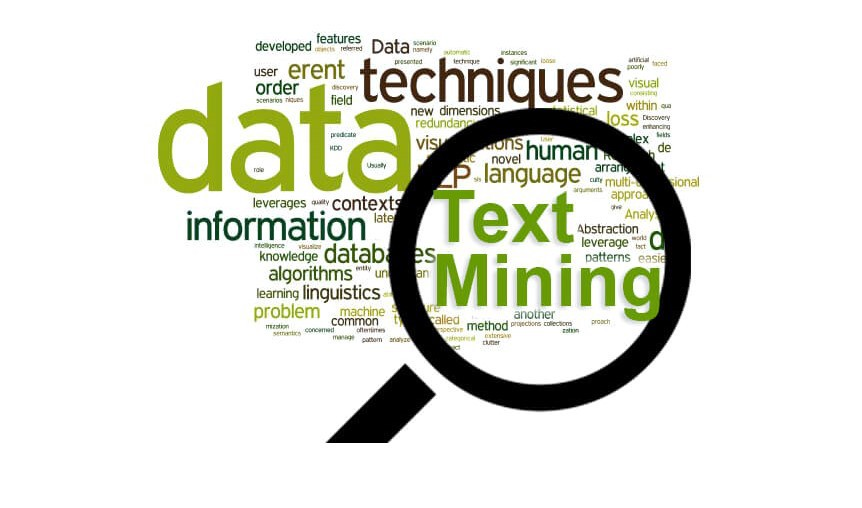
\includegraphics[width = 0.5 \textwidth]{fig31.jpg}}
\caption{Text mining.}
\label{fig31}
\end{figure}

Se estima que el 80\% de la información relevante para una empresa viene de algún tipo de datos no estructurados, los cuales están formados, en gran parte, por texto. Por ejemplo, podemos encontrar información relevante en e-mails, informes e, incluso, artículos en las redes sociales.



\subsection{Ventajas del Text Analytics}

\subsubsection{Estado real de la empresa}

En los textos redactados también entran los informes periódicos o los balances, por citar dos ejemplos. Repasando la información recopilada resulta más fácil descubrir el estado real de la empresa, por lo que es más sencillo adelantarse a posibles problemas y tomar decisiones acertadas \cite{Ormeno}.

\subsubsection{Opiniones en los clientes}

En el repaso de los textos también se incluyen las opiniones de los clientes, por lo que es posible determinar cuáles son los errores que se están cometiendo. Además, es posible personalizar la oferta comercial al entender mejor cuáles son sus necesidades o qué demanda exactamente.

\subsubsection{Creación de etiquetas}

Contribuye a la creación de etiquetas que clasifiquen los productos a la venta dependiendo de su material, fabricante o peculiaridades, entre otros factores.

\begin{figure}[htbp]
\centerline{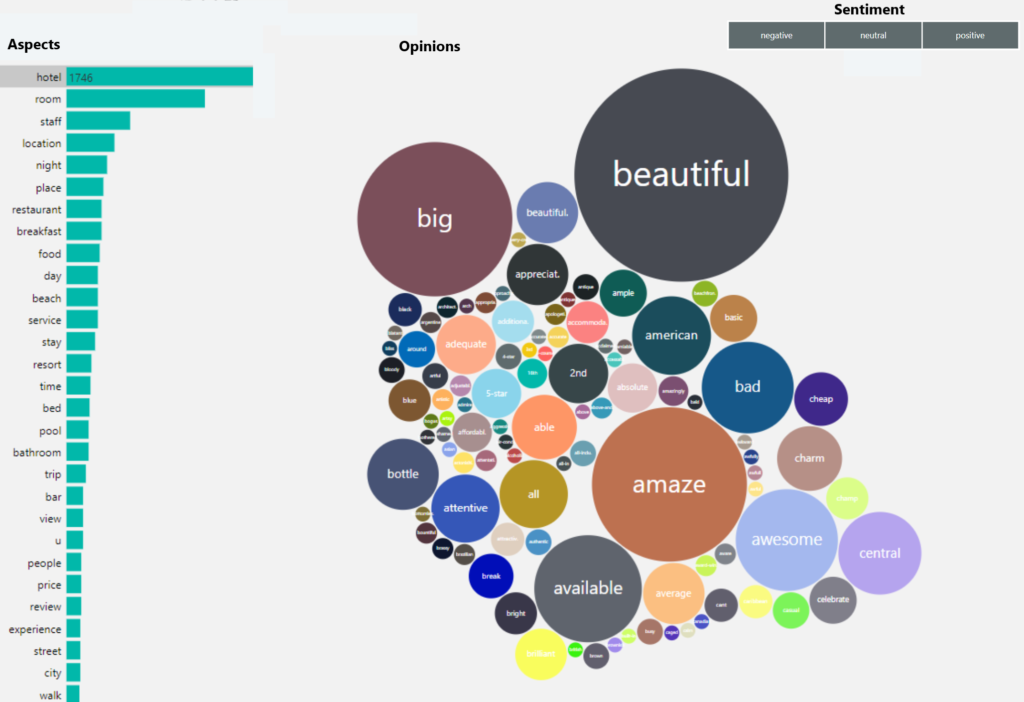
\includegraphics[width = 0.5 \textwidth]{fig44.png}}
\caption{Ejemplo de etiquetas.}
\label{fig44}
\end{figure}

Text Analytics (Text MIning), lo que parece ser una disciplina asociada a la Business Intelligence y al Big Data, es también una herramienta para predecir tendencias, conocer mejor a la clientela y, definitivamente, repasar la información pasada dándole su valor para convertirla en la más útil para el futuro.

\subsubsection{Speech Recognition}

El Reconocimiento Automático de Voz (RAH) o Reconocimiento Automático de Voz es un tema de inteligencia artificial, que tiene como objetivo realizar la comunicación de voz entre humanos y computadoras.

\begin{figure}[htbp]
\centerline{
\includegraphics[width = 0.5 \textwidth]{fig43.png}}
\caption{Reconocimiento de voz.}
\label{fig43}
\end{figure}

\subsubsection{En salud}

Encontrar información rápidamente a partir de registros médicos.
Las enfermeras pueden solicitar información administrativa, como el número de pacientes en un piso y el número de unidades disponibles.
En casa, los padres pueden preguntar por los síntomas comunes de las enfermedades, cuándo deben ir al médico y cómo cuidar a un niño enfermo.

\begin{figure}[htbp]
\centerline{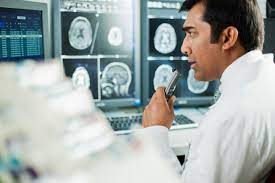
\includegraphics[width = 0.5 \textwidth]{fig38.jpg}}
\caption{Servicios cognitivos en salud.}
\label{fig38}
\end{figure}

\subsubsection{En banca}

Solicite información sobre su saldo, transacciones y hábitos de gasto sin tener que abrir su teléfono celular.
Realizar pagos.
Reciba información sobre su historial de transacciones.

\begin{figure}[htbp]
\centerline{
\includegraphics[width = 0.5 \textwidth]{fig42.jpg}}
\caption{Servicios cognitivos en banca.}
\label{fig42}
\end{figure}

\subsubsection{Con Internet de las cosas}

Aplicación de asistentes digitales en coches: 
Escuche mensajes con manos libres.
Controla tu radio.
Ayudar con la guía y la navegación.
Responder a los comandos de voz.

\begin{figure}[htbp]
\centerline{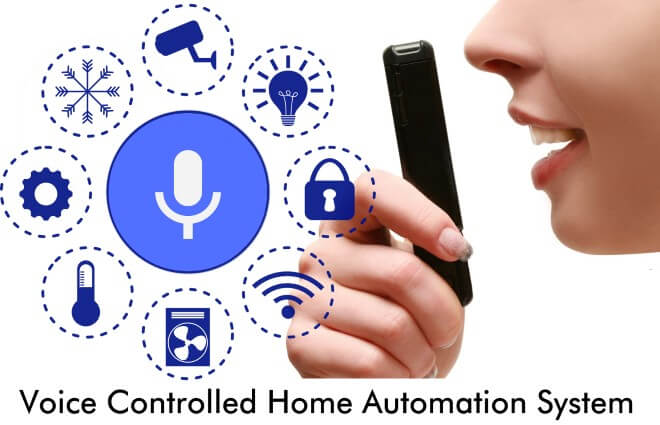
\includegraphics[width = 0.5 \textwidth]{fig33.jpg}}
\caption{Servicios cognitivos en IoT.}
\label{fig33}
\end{figure}

\subsubsection{Traducción}

La inteligencia artificial (IA) puede ayudar a simplificar la comunicación al traducir texto o habla entre idiomas, lo que ayuda a eliminar las barreras a la comunicación entre países y culturas.

\begin{figure}[htbp]
\centerline{
\includegraphics[width = 0.5 \textwidth]{fig37.png}}
\caption{Traductores y servicios cognitivos.}
\label{fig37}
\end{figure}

Traductor, parte de Servicios cognitivos Azure, es una nube basada en traducción automática servicio de apoyo a 90 idiomas y dialectos. Translator se puede utilizar para crear aplicaciones, sitios web, herramientas o cualquier solución que requiera soporte multilingüe.
¿Cómo funciona la traducción de voz?
Para traducir correctamente el discurso “fuente” de un idioma a otro idioma “target”, el sistema pasa por un proceso de cuatro pasos:

Reconocimiento de voz, convertir audio en texto.

TrueText: una tecnología de Microsoft que normaliza el texto para que sea más apropiado para la traducción.

Traducción a través del motor de traducción de texto descrito anteriormente, pero sobre modelos de traducción especialmente desarrollados para conversaciones habladas en la vida real.
Texto a voz, cuando sea necesario, para producir el audio traducido.

\begin{figure}[htbp]
\centerline{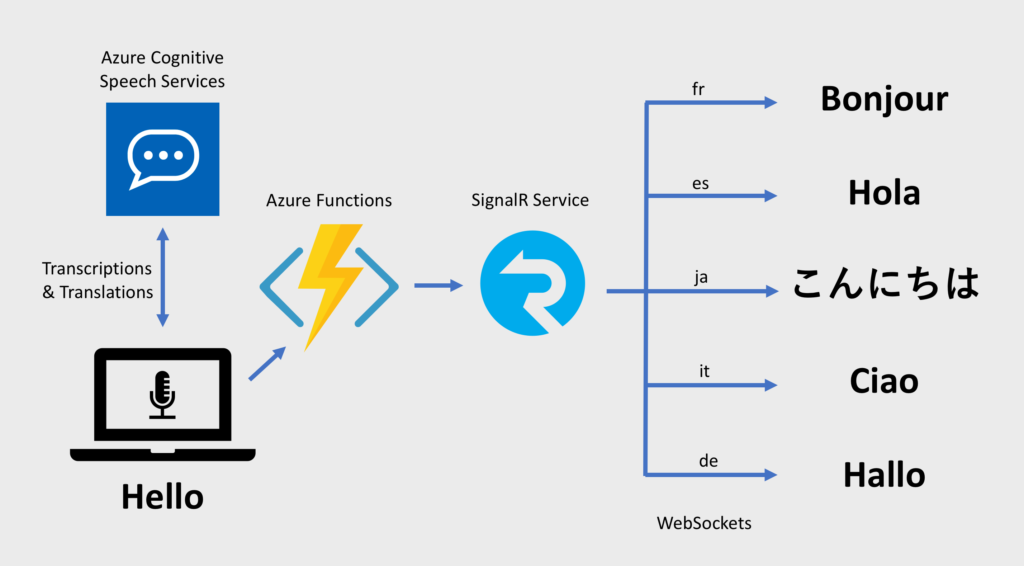
\includegraphics[width = 0.5 \textwidth]{fig32.png}}
\caption{Arquitectura de un traductor.}
\label{fig32}
\end{figure}

\subsubsection{Language Understanding (LUIS)}

Language Understanding Intelligent Service (LUIS, por sus siglas en inglés) utiliza el aprendizaje automático para permitir a los desarrolladores crear aplicaciones que puedan entender el lenguaje natural de los usuarios para extraer su significado y comprender lo que la persona quiere. En pocas palabras, tener la habilidad de entender de una manera clara la forma en que las personas se comunican en su cotidianidad.

\begin{figure}[htbp]
\centerline{
\includegraphics[width = 0.5 \textwidth]{fig39.jpg}}
\caption{LUIS}
\label{fig39}
\end{figure}

LUIS añade comprensión natural del lenguaje a tus aplicaciones. Está diseñado para identificar información valiosa en conversaciones, interpretar los objetivos del usuario e identificar información relevante en las oraciones para comunicarse en un lenguaje natural y de alta calidad.

LUIS está en constante aprendizaje. El aprendizaje de refuerzo se usa para mejorar continuamente la calidad de los modelos de procesamiento del lenguaje natural.

Una vez que el modelo comienza a procesar la entrada, la comprensión del idioma empieza su aprendizaje activo permitiendo así actualizar y mejorar constantemente el modelo.

Chatbot de información: Este Bot informacional puede responder preguntas definidas en un conjunto de conocimientos o preguntas frecuentes usando Azure Search.

Dispositivos de IoT: Se pueden crear interfaces de conversación con todos sus dispositivos accesibles en Internet.

\begin{figure}[htbp]
\centerline{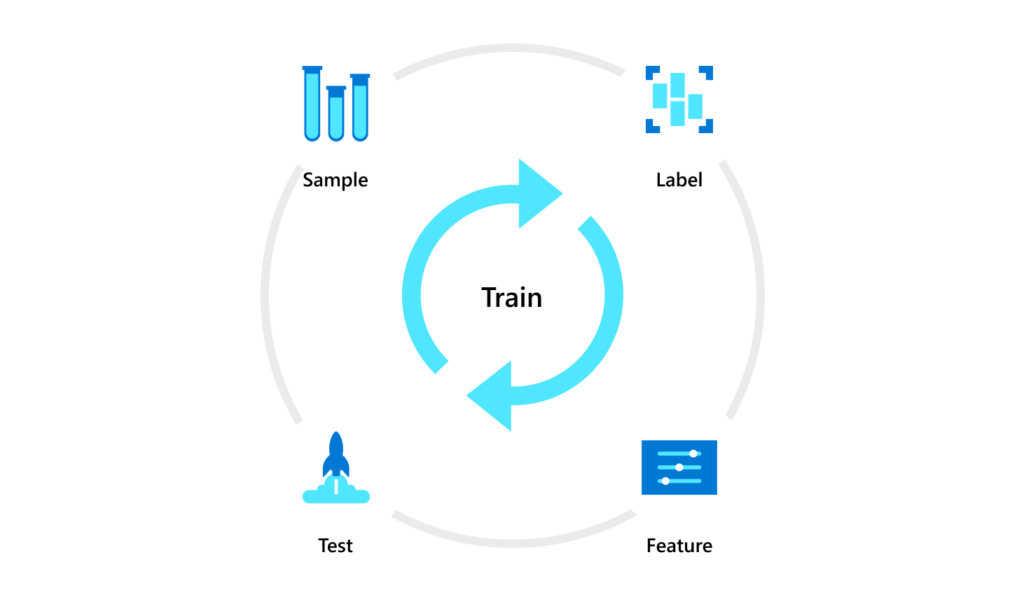
\includegraphics[width = 0.5 \textwidth]{fig40.png}}
\caption{Funcionamiento de LUIS}
\label{fig40}
\end{figure}

\subsubsection{Chatbot: ¿Qué es, para qué sirve y cómo funcionan?}

Hoy en día Internet está muy masificado, resulta difícil destacar entre tanta información. Las empresas buscan los canales digitales para llamar la atención y tener contacto con los usuarios. Los consumidores aceptan este hecho y prefieren tener el contacto con las empresas a través de mensajes.
Adiós a los medios digitales de antes, los medios tradicionales como los call center, por ejemplo, ya están obsoletos. La solución que se ha planteado para hacer feliz tanto a las empresas como a los consumidores son: los chatbots.

\begin{figure}[htbp]
\centerline{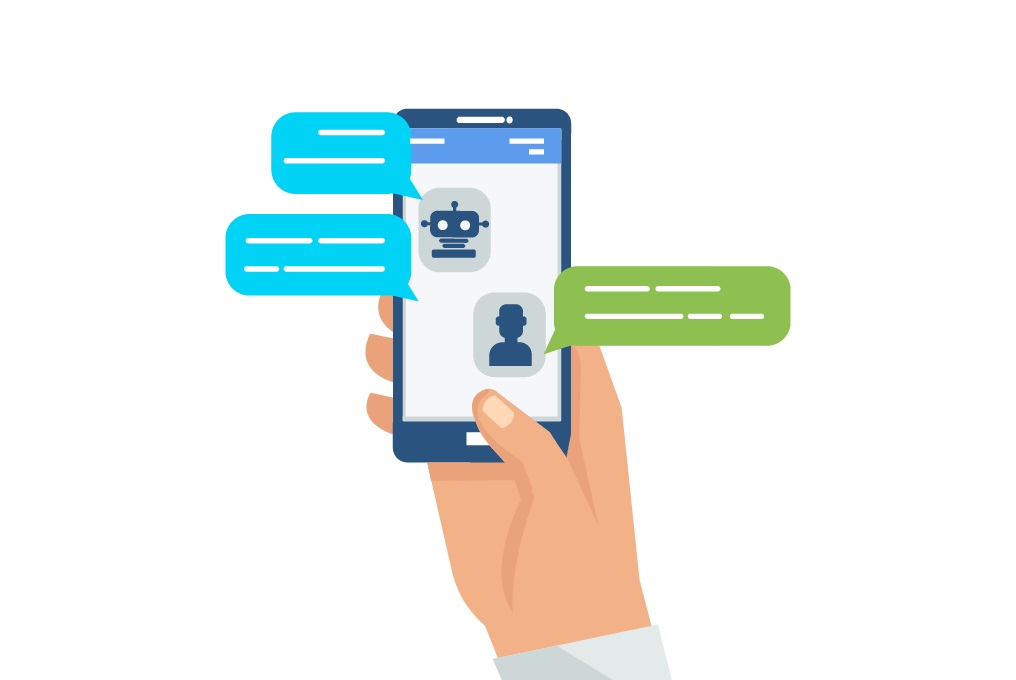
\includegraphics[width = 0.5 \textwidth]{fig41.jpg}}
\caption{Funcionamiento de un chatbot.}
\label{fig41}
\end{figure}

\subsubsection{¿Qué es un chatbot?}

De manera sencilla y comprensible podemos definir un chatbot como un asistente que se comunica con los usuarios a través de mensajes de texto. En muchas otras ocasiones, toma forma convirtiéndose en un compañero virtual que se integra en sitios web, aplicaciones, conversando y ayudando a los usuarios \cite{Peris}.

Se trata de una tecnología que permite al usuario mantener una conversación a través de un software que se integra en un determinado sistema de mensajería, como, por ejemplo: Facebook, Twitter, Telegram, Whatsapp, etc.
El sistema está programado para que interactúe con el cliente y le resuelva dudas, pero sin que haya una persona física contestando. Tienen la ventaja de que están disponibles siempre para resolver las dudas de los usuarios que quieran contactar contigo a cualquier hora del día.

Por lo tanto, estamos hablando de una herramienta que interactúa de manera automática con usuarios y potenciales clientes con el fin de guiarles hacia la acción deseada (conversión).

Los algoritmos desarrollados por la inteligencia artificial y de aprendizaje automático permiten que los chatbots sean capaces de aprender. Pueden llegar a intuir los hábitos y entender los gustos y preferencias de los usuarios.

Existen muchos tipos de chats en vivo, algunos de ellos ofrecen una experiencia tan auténtica, en la que es muy difícil determinar si el que contesta es un robot virtual o un ser humano.

\subsubsection{¿Por qué han aparecido los chatbots?}

Actualmente, estamos viviendo una transformación digital y un momento en el que los datos son un valor importante para las empresas. Es aquí donde entra el papel tan relevante de los chatbots, puesto que son softwares diseñados con el fin de poder conectar de manera personalizada con los usuarios, resolviendo sus dudas, aportando valor para ellos, pero disminuyendo enormemente el gasto que esta interacción supondría para la empresa si se realizara con representantes humanos. El resultado es un ahorro en tiempo y dinero para la empresa y una mayor comodidad y rapidez para el usuario.

\subsubsection{¿Cómo funcionan los chatbots?}

Para comprender el funcionamiento de un chatbot debemos primero entender qué es un bot. Un bot es un software de inteligencia artificial con la característica diferencial de ser capaz de realizar una serie de tareas por su cuenta, sin la ayuda del ser humano. 

El chatbot es un tipo de bot que interactúa con el usuario manteniendo conversaciones sencillas, pero que también puede convertirse en un sofisticado software a medida que procesan información, y aprender y evolucionar con el fin de ofrecer niveles de personalización cada vez más elevados. Siri y Cortana serían los ejemplos más conocidos de chatbot.

Los chatbots son utilizados por las empresas principalmente para llevar a cabo tareas y funciones de atención al cliente: realizar pedidos automáticos, comunicar incidencias técnicas, pedir información sobre un determinado producto o servicio, etc. Pero también tienen su uso en los procesos internos de la propia empresa, como pueden ser los pedidos de suministros internos, las programaciones en calendarios o facilitar el proceso de entrada de nuevos trabajadores.

La operatividad de los chatbots tiene lugar en las aplicaciones de mensajería, incorporando para ello un interfaz conversacional.
Vale la pena señalar que entender a los humanos no es fácil para una máquina. La forma sutil y matizada en la que nos comunicamos es una tarea muy compleja de recrear artificialmente, por lo que los chatbots utilizan varios principios del lenguaje natural:

\subsection{Procesamiento del Lenguaje Natural (PLN)}

El Procesamiento de Lenguaje Natural se utiliza para dividir la entrada del usuario en oraciones y palabras. También amplia el significado del texto a través de una serie de técnicas como, por ejemplo: Convirtiendo todo a minúsculas o corrigiendo errores ortográficos antes de determinar el significado de la palabra. En esta etapa, es donde también se consideran otros factores tales como las emociones del usuario.

\subsubsection{Comprensión del Lenguaje Natural (CLN)}

La comprensión del lenguaje natural ayuda al chatbot a entender lo que el usuario ha dicho, las herramientas que utiliza son tales como léxicos, sinónimos y temas. Estas herramientas son usadas en conjunto como algoritmos o reglas para construir el diálogo que le indicará al chatbot cómo debe responder de la mejor manera posible.

\subsubsection{Generación de Lenguaje Natural (GNL)}

Ofrecer una experiencia al cliente memorable, personalizada e ir más allá de brindar respuestas prefabricadas, requiere la generación de lenguaje natural. El chatbot puede consultar repositorios de datos y así, utilizar esa información para crear una respuesta.

La tecnología de IA Conversacional lleva el PLN y la CLN al siguiente nivel, permitiendo a las empresas puedan crear sistemas de diálogo avanzados.
Usan memorias y datos de preferencias personales y la propia comprensión contextual del chat para ofrecer una interfaz de lenguaje natural realista y atractiva.

\subsubsection{Ventajas de los chatbots}

Las principales ventajas del uso de chatbots por parte de las empresas son:

Permite ahorrar costes en formación y personal del departamento de atención al cliente.

Permite atender las principales dudas y gestiones de los usuarios de manera rápida.

Abre la posibilidad a escalar y a su vez ofrecer una atención personalizada, ya que se depende menos del esfuerzo humano, pero no es necesario usar modelos estandarizados para poder dar respuesta.

Un chatbot posibilita una interacción muy ágil con el cliente.

En ciertos casos, el chatbot puede llegar a proporcionar experiencias muy agradables y cómodas al usuario.

Otra ventaja es la rápida mejora de las posibilidades y el nivel de sofisticación de los softwares de inteligencia, llegando a simular con gran realismo conversaciones bastante complejas.

Se trata de una tecnología que está abriendo nuevas fuentes de ingresos y oportunidades de negocio. Por este motivo, desarrolladores de software, marcas y empresas se están volcando en ofrecer sus servicios a través de este canal.
A muchas personas les resulta más sencillo y cómodo hablar con un robot de voz que con la persona encargada de atenderle telefónicamente.
Tipos de chatbots que existen en el mercado
Actualmente, existen distintos tipos de chatbots que procesan la información y pueden dar respuesta a solicitudes de distinta índole. A continuación, explicamos los dos tipos principales de chatbots \cite{Escote}.

\subsubsection{Tipo 1 - Chatbots orientados a tareas (declarativos)}

Son programas que generan respuestas automatizadas a las consultas que los usuarios puedan realizar y lo hacen de manera conversacional. Es por ello que son más aplicables a los departamentos de soporte, atención al cliente y servicio, pues las interacciones con estos chatbots son específicas y estructuradas.

Los ejemplos más claros de chatbots declarativos serían aquellos que se emplean en preguntas comunes como precios de productos concretos u horarios comerciales. Sus capacidades son bastante básicas, pero son los chatbots más utilizados.

Tipo 2 - Chatbots basados en datos y predictivos (conversacionales)
Son herramientas capaces de personalizar su respuesta basándose en el perfil de cada usuario y su comportamiento anterior. Estos son conscientes del contexto y aprenden con cada nueva situación. Además, aprovechan su comprensión del lenguaje natural para ofrecer recomendaciones e incluso llegar a anticiparse a las necesidades del usuario.



¿Cómo crear un chatbot?
No es necesario ser un experto para crear un chatbot y hay muchas herramientas que permiten hacerlo. Crear uno es similar a desarrollar una aplicación móvil y se puede enfocar a usos empresariales o a consumidores.
Los chatbots se pueden crear e ir enfocados a ciertas herramientas. Por ejemplo, puedes crear un Chatbot para Whatsapp para mejorar el Customer Service de tu negocio.
Entre las distintas herramientas que existen en el mercado, con HubSpot puedes crear un Chatbot gratis para implementarlo en la web de tu empresa y enfocarlo como una parte más de tu estrategia de marketing.
El chatbot de Facebook
Aunque Twitter y otras plataformas, como Telegram, también han empezado a incorporar funciones de chatbots a sus servicios de mensajería, lo cierto es que de momento Facebook puede considerarse la empresa referente en el desarrollo de sistemas basados en chatbots.

Dado que la mayoría de las empresas no disponen de recursos propios para elaborar chatbots, Facebook les está suministrando herramientas de API (interfaz de programación de aplicaciones) para que puedan crear sus propios softwares de inteligencia artificial personalizados y adaptados a sus necesidades.

En Facebook, los chatbots se encuentran integrados dentro de su aplicación Messenger. Ello permite realizar acciones como encargar un ramo de flores o pedir que la CNN nos mande un resumen de las noticias que más nos interesan en función de nuestros gustos e inquietudes.
Se trata de una funcionalidad enfocada a empresas y marcas que el propio Mark Zuckerberg se encargó de promocionar en el último congreso de desarrolladores F8, afirmando que los usuarios podrán hablar con los chatbots igual que lo harían con sus amigos.  
Además de facilitar la atención al cliente y mejorar la experiencia del usuario, una ventaja adicional del chatbot de Facebook son las nuevas posibilidades publicitarias. La red social Facebook dará la opción a las empresas de enviar anuncios con mensajes patrocinados a aquellos usuarios que, previamente, hayan iniciado de manera voluntaria una conversación por chatbot con la marca.
Preguntas y Respuestas
¿Cuáles son los mejores chatbot?
Entre los mejores chatbots que se encuentran el mercado están:
Aivo
Zendesk
Botslover
Messenger People
Son plataformas que se pueden usar tanto en webs como en herramientas de mensajería, ofrecen herramientas de análisis y te permiten gestionar desde un solo espacio todos los canales que ofreces a tus usuarios.
¿Cuál es el mejor chatbot en español?
HubSpot actualmente se posiciona como la mejor herramienta para configurar un chatbot en español, pues permite mantener conversaciones a gran escala en el propio sitio web y automatizar los procesos. Así, tu equipo se focaliza en las conversaciones más importantes o delicadas. Es perfecto para empezar, pues no requiere ningún conocimiento técnico y dispone de plantillas con la opción de personalizarlas para alinearlo con la voz de tu marca. Asimismo, ayuda a calificar los leads y ofrecerles respuestas rápidas y adecuadas a las preguntas técnicas frecuentes y a hacer un seguimiento de las conversaciones.
¿Cuál es el mejor chatbot gratis para WhatsApp?
Zendesk es una aplicación chatbot gratuita y muy buena para usar en WhatsApp, pues te permite personalizar los mensajes, hacer seguimiento de las conversiones y permite tener un registro de toda la información que se recoge con el chatbot.
¿Dónde se utilizan los chatbots?
Los chatbots se pueden usar en 2 tipos de enfoque: a nivel interno o para interactuar con los consumidores.
En el ámbito del servicio al consumidor, podemos emplear los chatbots en la propia página web para dar respuesta a las dudas que tenga el usuario, y en las aplicaciones de mensajería o redes sociales para automatizar las conversaciones y agilizar procesos.
A nivel interno lo podemos usar para automatizar pedidos de suministros y otras tareas comunes como actualización de contraseñas, alertas en las oficinas o incorporación de nuevos trabajadores.
¿Qué son los chatbots en un móvil Android?
Un chatbot en Android es un software encargado de dar respuesta a las consultas que los usuarios de una App puedan tener. En la misma aplicación se despliega un chat donde el usuario puede lanzar consultas y hablar directamente con la empresa de la aplicación. Es una manera de ofrecer el servicio dentro de la propia aplicación, sin tener que sacar al usuario fuera de ésta.
¿Puede un chatbot funcionar sin IA?
Existen chatbots sin IA que se crean desde cero y permiten realizar tareas muy parecidas a los chatbots con inteligencia artificial. Estos son efectivos a la hora de mejorar el servicio al cliente, pero no captan todas las necesidades del cliente, ya que solo resuelven las dudas en las que ha habido una previa configuración.
¿Existen chatbots gratuitos?
Existen chatbots gratuitos que pueden ser muy útiles para un negocio que está empezando; entre ellos podemos encontrar:
Plataforma Centribal, que en su versión gratuita permite crear, gestionar y entrenar un chatbot.
Live Chat, que permite centralizar todas las conversaciones de la web en un solo sitio.
Zendesk, que es muy sencilla de instalar y permite integrar todo tipo de soportes, desde chat hasta redes sociales.

La Influencia de los sistemas cognitivos en la empresa
Desde un punto de vista conceptual genérico, hay dos grandes beneficios asociados a la utilización de sistemas cognitivos en las empresas: 
1) la racionalización y automatización de procesos.
2) el enriquecimiento de procesos, productos y servicios.
Desde el punto de vista de los casos de uso, los sistemas cognitivos tienen aplicación en cualquier industria y área funcional. Efectivamente, se basan en el reconocimiento de patrones a partir del procesamiento de un gran conjunto de datos a una escala que está más allá de la capacidad humana, con lo que se pueden aplicar en muchos dominios – como, por ejemplo, análisis e investigación de fraudes, recomendación y automatización de procesos de venta, sistemas de investigación y recomendación de gestión de calidad, agentes de servicio automatizados, sistemas automatizados de inteligencia y prevención de amenazas, sistemas de búsqueda y acceso a contenidos, etc \cite{Malhado}.
Tomemos como ejemplo detallado el sourcing y procurement; en particular, el proceso de source to settle. Típicamente, el 20\% de la inversión se concentra en el 80\% de los proveedores. Hay muchas transacciones, pero el valor monetario total de cada uno es bajo en comparación con el total y hay muchos proveedores potenciales para los bienes, por lo que el riesgo de oferta es también bajo. La automatización del proceso final (desde el aprovisionamiento hasta la contratación) para estas transacciones rutinarias de bajo riesgo (a través de la aplicación del aprendizaje automático y el procesamiento del lenguaje natural) libera personal cualificado para concentrarse en la inversión y proveedores con mayor riesgo de suministro y coste financiero, así como en la gestión de las relaciones con los proveedores más críticos. Y para estos procesos menos rutinarios, el aprendizaje automático aumenta el proceso de sourcing mediante el monitoreo de señales que podrían conducir a una interrupción del suministro, asesorando al personal sobre las acciones correctivas disponibles y alternativas. Todo el proceso (tanto rutinario como no rutinario) se implementa a través de una combinación de automatización y enriquecimiento. Todo esto significa otra cosa: que uno de los grandes impactos de los sistemas cognitivos está en la fuerza de trabajo. Ellos van a cambiar la fuerza de trabajo de las empresas. Ya no sorprende a nadie la predicción de que la fuerza de trabajo del futuro será compuesta no solo por humanos, sino también por agentes virtuales.

¿Qué deberían estar haciendo las empresas en torno al tema Sistemas Cognitivos / IA?
Existen varios modelos de utilización de capacidades cognitivas en las empresas:
Agentes cognitivos dedicados que pueden ser involucrados en varios procesos de la empresa.
Funcionalidades embebidas en el software empresarial.
Plataformas de servicios (típicamente consumidos a través de la nube).
Queda claro que cualquiera que sea la combinación o arquitectura seleccionada por cada empresa, esta implicará una revisión de sus procesos. El TI y el negocio tendrán que trabajar conjuntamente para evaluar el valor de la nueva inteligencia proporcionada por el software e identificar los casos de implementación prioritaria. Además, las empresas deberían estar buscando a sus proveedores de tecnología para ver cómo las capacidades cognitivas / IA están siendo incluidas en los roadmaps de productos y cómo podrán hacer uso de dichas capacidades. Y los departamentos de TI deberán estar aprendiendo sobre las diversas plataformas de software cognitivo / AI disponibles y comenzar a probar algunas nuevas aplicaciones en ellos. Algunas de estas plataformas son gratuitas para uso en desarrollo. Las organizaciones de TI necesitan crear experiencia interna en estas áreas junto con la ciencia de datos y Big Data.

Servicios cognitivos y su impacto en la empresa Microsoft
Los servicios cognitivos de Microsoft son API basadas en la nube que puede usar en aplicaciones de inteligencia artificial (AI) y flujos de datos. Proporcionan modelos previamente entrenados que están listos para usarlos en cualquier aplicación, no requieren datos ni entrenamiento del modelo por su parte. Los servicios cognitivos los desarrolla el equipo de inteligencia artificial e investigación de Microsoft y aprovechan los algoritmos de aprendizaje profundo más recientes. Se consumen a través de las interfaces de REST de HTTP. Además, hay disponibles SDK para muchos marcos de desarrollo de aplicaciones comunes \cite{Microsoft2022}.
Los servicios cognitivos incluyen:
Análisis de texto
Visión del equipo
Análisis de vídeo
Reconocimiento y generación de voz
Comprensión del lenguaje natural
Búsqueda inteligente
Ventajas principales:
Con un esfuerzo mínimo de desarrollo se logran servicios de AI de última generación.
Fácil integración en aplicaciones a través de interfaces de REST de HTTP.
Compatibilidad integrada para consumir servicios cognitivos en Azure Data Lake Analytics.
Consideraciones:

Solo está disponible a través de Internet. Por lo general se requiere conectividad a Internet. Una excepción es Custom Vision Service, cuyo modelo entrenado se puede exportar para la predicción en dispositivos y en el borde de IoT.

Aunque se admite una personalización considerable, es posible que los servicios disponibles no se ajusten a todos los requisitos de análisis predictivo.

¿Qué opciones tiene al elegir entre los servicios cognitivos?
En Azure, existen docenas de servicios cognitivos disponibles. La lista actual de ellos está disponible en un directorio y están clasificados por el área funcional que admiten:
Visión
Identifique y analice el contenido de imágenes y vídeos
API de reconocimiento facial: Detecte e identifique a personas y emoticonos en las imágenes.

Computer Vision: Analice el contenido de imágenes y vídeos.

Custom Vision: Personalice el reconocimiento de imágenes para adaptarlo a sus necesidades empresariales.
Voz 
Mejore las experiencias de los clientes con Cognitive Service para voz:
Speech to Text: Transcriba la vox en texto legible en el que se puedan realizar búsquedas.

Text to Speech: Convierta el texto en un lenguaje más real para obtener interfaces más naturales.

Speech Translation: Integre fácilmente traducción de voz en tiempo real en sus aplicaciones.

Speaker Recognition: Identifique a las personas que hablan y compruébelo basándose en audio.
Decisión
Tome decisiones más inteligentes en menos tiempo
Anomaly Detector: Realice una identificación temprana de los posibles problemas.

Content Moderator: Detecte contenido potencialmente ofensivo o no deseado.

Personalizer: Cree experiencias personalizadas muy completas para cada usuario.
Lenguaje
Entienda las conversaciones y el texto no estructurado con Cognitive Service para lenguaje:
Reconocimiento de entidades: Identifique los términos de uso común y específicos del dominio \cite{Molnar2019}.

Análisis de opiniones: Detecte automáticamente sentimientos y opiniones a partir de texto.

Respuesta a preguntas: Cree una capa conversacional de preguntas y respuestas sobre los datos.

Language Understanding: Incorpore reconocimiento del lenguaje natural a sus aplicaciones, bots y dispositivos IoT.

Translator Text: Detecte y traduzca más de 100 idiomas y dialectos.
OpenAI
Modelos de lenguaje dinámicos para mejorar las aplicaciones
OpenAI Service: Aplique modelos de lenguaje avanzados a una gran variedad de casos de uso.

Principales criterios de selección
Para restringir las opciones, empiece por responder a estas preguntas:

¿Con qué tipo de datos trata? Puede limitar las opciones en función del tipo de datos de entrada con el que trabaje. Por ejemplo, si la entrada es texto, seleccione uno de los servicios que tenga un tipo de entrada de texto.

¿Tiene los datos necesarios para entrenar un modelo? En caso afirmativo, considere los servicios personalizados que le permiten entrenar sus modelos subyacentes con los datos que proporcione, con el fin de mejorar la precisión y el rendimiento \cite{Blanco}.

Matriz de funcionalidades
En las tablas siguientes se resumen las diferencias clave en cuanto a funcionalidades.

Usa modelos creados previamente
\begin{table}[]
\begin{tabular}{| p{0.15\linewidth} | p{0.15\linewidth} | p{0.5\linewidth} |}
\hline
\textbf{Capacidad} &
  \textbf{Tipo de entrada} &
  \textbf{Principal ventaja} \\ \hline
Text Analytics API &
  Texto &
  Evalúe las opiniones y temas para comprender lo que los usuarios quieren. \\ \hline
Entity Linking API &
  Texto &
  Alimente los vínculos de datos de su aplicación con el reconocimiento y la anulación de ambigüedades de las entidades con nombre. \\ \hline
Language Understanding Intelligent Service (LUIS) &
  Texto &
  Enseñe a las aplicaciones a entender los comandos de los usuarios. \\ \hline
Servicio QnA Maker &
  Texto &
  Convierta la información con formato de preguntas frecuentes en respuestas conversacionales por las que sea fácil navegar. \\ \hline
Linguistic Analysis API &
  Texto &
  Simplifique conceptos complejos del lenguaje y analice el texto. \\ \hline
Servicio Knowledge Exploration &
  Texto &
  Permita experiencias de búsqueda interactiva a través de datos estructurados mediante entradas en lenguaje natural. \\ \hline
Web Language Model API &
  Texto &
  Use modelos de lenguaje predictivos entrenados con datos de escala web. \\ \hline
Academic Knowledge API &
  Texto &
  Descubra la riqueza del contenido académico de Microsoft Academic Graph rellenado por Bing. \\ \hline
Bing Autosuggest API &
  Texto &
  Proporcione a su aplicación opciones de sugerencias automáticas inteligentes para las búsquedas. \\ \hline
Bing Spell Check API &
  Texto &
  Detecte y corrija errores ortográficos en las aplicaciones. \\ \hline
Translator Text API &
  Texto &
  Servicio de traducción automática. \\ \hline
Recommendations API &
  Texto &
  Prediga y recomiende los artículos que sus clientes quieren. \\ \hline
Bing Entity Search API &
  Texto (consulta de búsqueda web) &
  Identifique y amplíe la información de las entidades desde la web. \\ \hline
Bing Image Search API &
  Texto (consulta de búsqueda web) &
  Busque imágenes. \\ \hline
Bing News Search API &
  Texto (consulta de búsqueda web) &
  Busque noticias. \\ \hline
Bing Video Search API &
  Texto (consulta de búsqueda web) &
  Busque vídeos. \\ \hline
Bing Web Search API &
  Texto (consulta de búsqueda web) &
  Obtenga detalles mejorados de la búsqueda de miles de millones de documentos web. \\ \hline
Bing Speech API &
  Texto o voz &
  Convierta voz en texto, y viceversa. \\ \hline
Speaker Recognition API &
  Voz &
  Use la voz para identificar y autenticar a hablantes individuales. \\ \hline
Translator Speech API &
  Voz &
  Realice traducciones de voz en tiempo real. \\ \hline
\end{tabular}
\end{table}

\begin{table}[]
\begin{tabular}{| p{0.15\linewidth} | p{0.15\linewidth} | p{0.55\linewidth} |}
\hline
\textbf{Capacidad} &
  \textbf{Tipo de entrada} &
  \textbf{Principal ventaja} \\ \hline
Computer Vision API &
  Imágenes (o fotogramas de vídeo) &
  Convierta la información accionable de las imágenes, cree automáticamente la descripción de las fotos, derive etiquetas, reconozca a celebridades, extraiga texto y cree miniaturas precisas. \\ \hline
Content Moderator &
  Texto, imágenes o vídeo &
  Moderación automatizada de imágenes, texto y vídeo. \\ \hline
Emotion API &
  Imágenes (fotos con seres humanos) &
  Identifique la gama de emociones de los seres humanos. \\ \hline
Face API &
  Imágenes (fotos con seres humanos) &
  Detecte, identifique, analice, organice y etiquete las caras en las fotos. \\ \hline
Video Indexer &
  Vídeo &
  Información acerca del vídeo, como la opinión, transcriba la voz, traduzca la voz, reconozca caras y emociones, y extraiga las palabras clave. \\ \hline
\end{tabular}
\end{table}
\section{Propuestas}
\section{Conclusiones}
El presente trabajo partió con la premisa de investigar el impacto de los servicios cognitivos en la gestión del conocimiento, para ello, primero definimos qué son dichos servicios cognitivos, desde un punto de vista teórico, es decir las áreas de la inteligencia artificial asociados a ellos; pero también desde un punto de vista comercial, identificando a los principales actores que ofrecen éstos servicios como un producto que ya tiene un nivel de adopción alto, como Microsoft Azure Cognitive Services e IBM Watson.
Encontramos que las aplicaciones que se le da a ésta tecnología en las empresas, especialmente de la región, tiene un profundo impacto en el acceso al conocimiento de las organizaciones, pues, uno de los principales servicios es el de búsqueda, permitiendo simplificar y minimizar el esfuerzo para clasificar las enormes moles de conocimiento, que tradicionalmente requiere hacerse a mano. Con los servicios cognitivos, se puede organizar dicha información y ponerla a disposición usando servicios de búsqueda simples de usar, pero tremendamente sofisticados internamente.
Finalmente esbozamos un vistazo a un futuro, de momento hipotético, en el que los servicios cognitivos, junto con otras tecnologías como ontologías, agentes para tareas complejas, entre otras, podrían ser usadas en conjunto para construir agentes que no solo utilicen el conocimiento de una organización, no solamente lo hagan disponible para las personas, sino que también produzca nuevo conocimiento e incluso se puedan desempeñar con mínima supervisión humana en tareas críticas de apoyo a la toma de decisiones. 

\bibliographystyle{ieeetr}
\bibliography{bibliography.bib}

\end{document}